\section{Iterative Bayesian Unfolding}
\label{app:IBU}

As a cross-check and comparison, Iterative Bayesian Unfolding (IBU) (described in section~\ref{sec:UnfoldIntro}) using the \texttt{RooUnfold} package~\cite{Adye:2011gm} was performed. At present, this is done using the detector response of the \powheg+\pythia~samples to unfold reconstructed events from the \sherpa~2.2.1 samples with $\pTll > 190$~GeV, analogous to what has been done in the analysis up to this point.

First, various plots for the efficiency and purity of the \powheg+\pythia~sample are shown, and the results of the unfolding are shown in the following section.

\subsection{Relevant quantities and choice of binning}
The efficiency, or the correction factor \textbf{c} as defined in section~\ref{sec:UnfoldIntro}, describes the probability that an event that fulfills the fiducial requirement passes the analysis selection. This can be written as,
\begin{equation}
  \varepsilon_i=\frac{N^{\text{truth$_i$, reco}}}{N^{\text{truth$_i$}}}
\end{equation}
where $N^{\text{truth$_i$, reco}}$ represents the number of events in truth bin $i$ that pass the analysis selection, and $N^{\text{truth$_i$}}$ is the total number of truth events in bin $i$. The purity describes the probability that an event reconstructed in bin $i$ also falls in truth bin $i$. This can be written as:

\begin{equation}
  P_i=\frac{N^{\text{reco$_i$, truth$_i$}}}{N^{\text{reco$_i$}}}
\end{equation}
where $N^{\text{reco$_i$, truth$_i$}}$ represents the number of reconstructed events in bin $i$ with a truth event also in bin $i$, and $N^{\text{reco$_i$}}$ represents the total reconstructed events in bin $i$.

Lastly, the fake factor \textbf{f} as defined in section~\ref{sec:UnfoldIntro} describes the probability that a reconstructed event in bin $i$ also passes the fiducial selection. It can be written as:

\begin{equation}
  \textbf{f}_i = \frac{N^{\text{reco$_i$, truth}}}{N^{\text{reco$_i$}}}
\end{equation}

Figure~\ref{fig:EffDilep},~\ref{fig:EffTJ1} and~\ref{fig:EffTJ2} shows the efficiency measurements for the 24 variables that were outlined for UniFold and MultiFold, and figure~\ref{fig:binPurDilep},~\ref{fig:binPurTJ1}, and~\ref{fig:binPurTJ2} shows the purity for the same variables. Figures~\ref{fig:ffDilep},~\ref{fig:ffTJ1}, and~\ref{fig:ffTJ2} show the fake factor.

\begin{figure}[h!]
  \centering
  \includegraphics[page=443,width=0.45\textwidth]{figures/UnfoldingRelatedPlots.pdf}
  \includegraphics[page=447,width=0.45\textwidth]{figures/UnfoldingRelatedPlots.pdf} \\
  \includegraphics[page=455,width=0.45\textwidth]{figures/UnfoldingRelatedPlots.pdf}
  \includegraphics[page=459,width=0.45\textwidth]{figures/UnfoldingRelatedPlots.pdf} \\
  \includegraphics[page=463,width=0.45\textwidth]{figures/UnfoldingRelatedPlots.pdf}
  \includegraphics[page=467,width=0.45\textwidth]{figures/UnfoldingRelatedPlots.pdf} \\
  \includegraphics[page=471,width=0.45\textwidth]{figures/UnfoldingRelatedPlots.pdf}
  \includegraphics[page=475,width=0.45\textwidth]{figures/UnfoldingRelatedPlots.pdf} \\
  \caption{Efficiency as a function of $\pTll$, $\yll$, and $\pt$, $\eta$, and $\phi$ for the leading and subleading muon. This quantity estimates the probability that an event which passes the fiducial selection also passes the analysis selection.}
  \label{fig:EffDilep}
\end{figure}

\begin{figure}[h!]
  \centering
  \includegraphics[page=479,width=0.45\textwidth]{figures/UnfoldingRelatedPlots.pdf}
  \includegraphics[page=507,width=0.45\textwidth]{figures/UnfoldingRelatedPlots.pdf} \\
  \includegraphics[page=483,width=0.45\textwidth]{figures/UnfoldingRelatedPlots.pdf}
  \includegraphics[page=511,width=0.45\textwidth]{figures/UnfoldingRelatedPlots.pdf} \\
  \includegraphics[page=487,width=0.45\textwidth]{figures/UnfoldingRelatedPlots.pdf}
  \includegraphics[page=515,width=0.45\textwidth]{figures/UnfoldingRelatedPlots.pdf} \\
  \includegraphics[page=535,width=0.45\textwidth]{figures/UnfoldingRelatedPlots.pdf}
  \includegraphics[page=539,width=0.45\textwidth]{figures/UnfoldingRelatedPlots.pdf}
  \caption{Efficiency as a function $\pt$, $y$, $\phi$, and $n_{\text{ch}}$ for the leading and subleading track jet.}
  \label{fig:EffTJ1}
\end{figure}

\begin{figure}[h!]
  \centering
  \includegraphics[page=491,width=0.45\textwidth]{figures/UnfoldingRelatedPlots.pdf}
  \includegraphics[page=519,width=0.45\textwidth]{figures/UnfoldingRelatedPlots.pdf} \\
  \includegraphics[page=495,width=0.45\textwidth]{figures/UnfoldingRelatedPlots.pdf}
  \includegraphics[page=523,width=0.45\textwidth]{figures/UnfoldingRelatedPlots.pdf} \\
  \includegraphics[page=499,width=0.45\textwidth]{figures/UnfoldingRelatedPlots.pdf}
  \includegraphics[page=527,width=0.45\textwidth]{figures/UnfoldingRelatedPlots.pdf} \\
  \includegraphics[page=503,width=0.45\textwidth]{figures/UnfoldingRelatedPlots.pdf}
  \includegraphics[page=531,width=0.45\textwidth]{figures/UnfoldingRelatedPlots.pdf}
  \caption{Efficiency as a function for $m$, $\tau_1$, $\tau_2$, and $\tau_3$ for the leading and subleading track jet.}
  \label{fig:EffTJ2}
\end{figure}

\begin{figure}[h!]
  \centering
  \includegraphics[page=444,width=0.45\textwidth]{figures/UnfoldingRelatedPlots.pdf}
  \includegraphics[page=448,width=0.45\textwidth]{figures/UnfoldingRelatedPlots.pdf} \\
  \includegraphics[page=456,width=0.45\textwidth]{figures/UnfoldingRelatedPlots.pdf}
  \includegraphics[page=460,width=0.45\textwidth]{figures/UnfoldingRelatedPlots.pdf} \\
  \includegraphics[page=464,width=0.45\textwidth]{figures/UnfoldingRelatedPlots.pdf}
  \includegraphics[page=468,width=0.45\textwidth]{figures/UnfoldingRelatedPlots.pdf} \\
  \includegraphics[page=472,width=0.45\textwidth]{figures/UnfoldingRelatedPlots.pdf}
  \includegraphics[page=476,width=0.45\textwidth]{figures/UnfoldingRelatedPlots.pdf}
  \caption{Purity for $\pTll$, $\yll$, and $\pt$, $\eta$, and $\phi$ for the leading and subleading muon. This quantity provides the probability that an event in a given reconstructed bin occurs in the same truth bin.}
  \label{fig:binPurDilep}
\end{figure}

\begin{figure}[h!]
  \centering
  \includegraphics[page=480,width=0.45\textwidth]{figures/UnfoldingRelatedPlots.pdf}
  \includegraphics[page=508,width=0.45\textwidth]{figures/UnfoldingRelatedPlots.pdf} \\
  \includegraphics[page=484,width=0.45\textwidth]{figures/UnfoldingRelatedPlots.pdf}
  \includegraphics[page=512,width=0.45\textwidth]{figures/UnfoldingRelatedPlots.pdf} \\
  \includegraphics[page=488,width=0.45\textwidth]{figures/UnfoldingRelatedPlots.pdf}
  \includegraphics[page=516,width=0.45\textwidth]{figures/UnfoldingRelatedPlots.pdf} \\
  \includegraphics[page=536,width=0.45\textwidth]{figures/UnfoldingRelatedPlots.pdf}
  \includegraphics[page=540,width=0.45\textwidth]{figures/UnfoldingRelatedPlots.pdf}
  \caption{Purity for $\pt$, $y$, $\phi$, and $n_{\text{ch}}$ for the leading and subleading track jet.}
  \label{fig:binPurTJ1}
\end{figure}

\begin{figure}[h!]
  \centering
  \includegraphics[page=492,width=0.45\textwidth]{figures/UnfoldingRelatedPlots.pdf}
  \includegraphics[page=520,width=0.45\textwidth]{figures/UnfoldingRelatedPlots.pdf} \\
  \includegraphics[page=496,width=0.45\textwidth]{figures/UnfoldingRelatedPlots.pdf}
  \includegraphics[page=524,width=0.45\textwidth]{figures/UnfoldingRelatedPlots.pdf} \\
  \includegraphics[page=500,width=0.45\textwidth]{figures/UnfoldingRelatedPlots.pdf}
  \includegraphics[page=528,width=0.45\textwidth]{figures/UnfoldingRelatedPlots.pdf} \\
  \includegraphics[page=504,width=0.45\textwidth]{figures/UnfoldingRelatedPlots.pdf}
  \includegraphics[page=532,width=0.45\textwidth]{figures/UnfoldingRelatedPlots.pdf}
  \caption{Purity for $m$, $\tau_1$, $\tau_2$, and $\tau_3$ for the leading and subleading track jet.}
  \label{fig:binPurTJ2}
\end{figure}

The purity values are the relevant quantity used to determine if the chosen binning is appropriate for a given variable. Ideally, each bin will have a purity of $\sim$60\%--70\%. The bins chosen for each variable are outlined in table~\ref{tab:IBUBins}.

\begin{figure}[h!]
  \centering
  \includegraphics[page=445,width=0.45\textwidth]{figures/UnfoldingRelatedPlots.pdf}
  \includegraphics[page=449,width=0.45\textwidth]{figures/UnfoldingRelatedPlots.pdf} \\
  \includegraphics[page=457,width=0.45\textwidth]{figures/UnfoldingRelatedPlots.pdf}
  \includegraphics[page=461,width=0.45\textwidth]{figures/UnfoldingRelatedPlots.pdf} \\
  \includegraphics[page=465,width=0.45\textwidth]{figures/UnfoldingRelatedPlots.pdf}
  \includegraphics[page=469,width=0.45\textwidth]{figures/UnfoldingRelatedPlots.pdf} \\
  \includegraphics[page=473,width=0.45\textwidth]{figures/UnfoldingRelatedPlots.pdf}
  \includegraphics[page=477,width=0.45\textwidth]{figures/UnfoldingRelatedPlots.pdf}
  \caption{Fake factor for $\pTll$, $\yll$, and $\pt$, $\eta$, and $\phi$ for the leading and subleading muon. This quantity provides the probability that an event in a given reconstructed bin occurs in the same truth bin.}
  \label{fig:ffDilep}
\end{figure}

\begin{figure}[h!]
  \centering
  \includegraphics[page=481,width=0.45\textwidth]{figures/UnfoldingRelatedPlots.pdf}
  \includegraphics[page=509,width=0.45\textwidth]{figures/UnfoldingRelatedPlots.pdf} \\
  \includegraphics[page=485,width=0.45\textwidth]{figures/UnfoldingRelatedPlots.pdf}
  \includegraphics[page=513,width=0.45\textwidth]{figures/UnfoldingRelatedPlots.pdf} \\
  \includegraphics[page=489,width=0.45\textwidth]{figures/UnfoldingRelatedPlots.pdf}
  \includegraphics[page=517,width=0.45\textwidth]{figures/UnfoldingRelatedPlots.pdf} \\
  \includegraphics[page=537,width=0.45\textwidth]{figures/UnfoldingRelatedPlots.pdf}
  \includegraphics[page=541,width=0.45\textwidth]{figures/UnfoldingRelatedPlots.pdf}
  \caption{Fake factor for $\pt$, $y$, $\phi$, and $n_{\text{ch}}$ for the leading and subleading track jet.}
  \label{fig:ffTJ1}
\end{figure}

\begin{figure}[h!]
  \centering
  \includegraphics[page=493,width=0.45\textwidth]{figures/UnfoldingRelatedPlots.pdf}
  \includegraphics[page=521,width=0.45\textwidth]{figures/UnfoldingRelatedPlots.pdf} \\
  \includegraphics[page=497,width=0.45\textwidth]{figures/UnfoldingRelatedPlots.pdf}
  \includegraphics[page=525,width=0.45\textwidth]{figures/UnfoldingRelatedPlots.pdf} \\
  \includegraphics[page=501,width=0.45\textwidth]{figures/UnfoldingRelatedPlots.pdf}
  \includegraphics[page=529,width=0.45\textwidth]{figures/UnfoldingRelatedPlots.pdf} \\
  \includegraphics[page=505,width=0.45\textwidth]{figures/UnfoldingRelatedPlots.pdf}
  \includegraphics[page=533,width=0.45\textwidth]{figures/UnfoldingRelatedPlots.pdf}
  \caption{Purity for $m$, $\tau_1$, $\tau_2$, and $\tau_3$ for the leading and subleading track jet.}
  \label{fig:ffTJ2}
\end{figure}

The response matrices, which are also defined in section~\ref{sec:UnfoldIntro}, are shown in figure~\ref{fig:migMatDilep},~\ref{fig:migMatTJ1}, and~\ref{fig:migMatTJ2}.

\begin{figure}[h!]
  \centering
  \includegraphics[page=558,width=0.45\textwidth]{figures/UnfoldingRelatedPlots.pdf}
  \includegraphics[page=559,width=0.45\textwidth]{figures/UnfoldingRelatedPlots.pdf} \\
  \includegraphics[page=561,width=0.45\textwidth]{figures/UnfoldingRelatedPlots.pdf}
  \includegraphics[page=562,width=0.45\textwidth]{figures/UnfoldingRelatedPlots.pdf} \\
  \includegraphics[page=563,width=0.45\textwidth]{figures/UnfoldingRelatedPlots.pdf}
  \includegraphics[page=564,width=0.45\textwidth]{figures/UnfoldingRelatedPlots.pdf} \\
  \includegraphics[page=565,width=0.45\textwidth]{figures/UnfoldingRelatedPlots.pdf}
  \includegraphics[page=566,width=0.45\textwidth]{figures/UnfoldingRelatedPlots.pdf}
  \caption{The response matrices for $\pTll$, $\yll$, and $\pt$, $\eta$, and $\phi$ for the leading and subleading muon.}
  \label{fig:migMatDilep}
\end{figure}

\begin{figure}[h!]
  \centering
  \includegraphics[page=567,width=0.45\textwidth]{figures/UnfoldingRelatedPlots.pdf}
  \includegraphics[page=574,width=0.45\textwidth]{figures/UnfoldingRelatedPlots.pdf} \\
  \includegraphics[page=568,width=0.45\textwidth]{figures/UnfoldingRelatedPlots.pdf}
  \includegraphics[page=575,width=0.45\textwidth]{figures/UnfoldingRelatedPlots.pdf} \\
  \includegraphics[page=569,width=0.45\textwidth]{figures/UnfoldingRelatedPlots.pdf}
  \includegraphics[page=576,width=0.45\textwidth]{figures/UnfoldingRelatedPlots.pdf} \\
  \includegraphics[page=581,width=0.45\textwidth]{figures/UnfoldingRelatedPlots.pdf}
  \includegraphics[page=582,width=0.45\textwidth]{figures/UnfoldingRelatedPlots.pdf}
  \caption{The response matrices for $\pt$, $y$, $\phi$, and $n_{\text{ch}}$ for the leading and subleading track jet.}
  \label{fig:migMatTJ1}
\end{figure}

\begin{figure}[h!]
  \centering
  \includegraphics[page=570,width=0.45\textwidth]{figures/UnfoldingRelatedPlots.pdf}
  \includegraphics[page=577,width=0.45\textwidth]{figures/UnfoldingRelatedPlots.pdf} \\
  \includegraphics[page=571,width=0.45\textwidth]{figures/UnfoldingRelatedPlots.pdf}
  \includegraphics[page=578,width=0.45\textwidth]{figures/UnfoldingRelatedPlots.pdf} \\
  \includegraphics[page=572,width=0.45\textwidth]{figures/UnfoldingRelatedPlots.pdf}
  \includegraphics[page=579,width=0.45\textwidth]{figures/UnfoldingRelatedPlots.pdf} \\
  \includegraphics[page=573,width=0.45\textwidth]{figures/UnfoldingRelatedPlots.pdf}
  \includegraphics[page=580,width=0.45\textwidth]{figures/UnfoldingRelatedPlots.pdf}
  \caption{The response matrices for $m$, $\tau_1$, $\tau_2$, and $\tau_3$ for the leading and subleading track jet.}
  \label{fig:migMatTJ2}
\end{figure}

\subsection{Efficiency studies}

As can be seen in Figure~\ref{fig:EffDilep}, there is a drop in efficiency at higher values of the inidividual muon \pt and $\pTll$. This is a result of \pt misreconstruction for higher \pt muons, which results in the dilepton mass falling out of acceptance.
The resolution plots for $\pTll$ and $m_{\mu\mu}$ can be seen in Figure~\ref{fig:Resmll}.

\begin{figure}
  \centering
  \includegraphics[page=587,width=0.45\textwidth]{figures/UnfoldingRelatedPlots.pdf}
  \includegraphics[page=588,width=0.45\textwidth]{figures/UnfoldingRelatedPlots.pdf}
  \includegraphics[page=1175,width=0.45\textwidth]{figures/UnfoldingRelatedPlots.pdf}
  \includegraphics[page=1176,width=0.45\textwidth]{figures/UnfoldingRelatedPlots.pdf}
  %\caption{The ratio of reconstructed $m_{\mu\mu}$ to truth $m_{\mu\mu}$ for \powheg+\pythia~(top left) and \sherpa~2.2.1 (bottom left), and similarly for $\pTll$ (right).}
  \caption{The detector resolution of $m_{\mu\mu}$ (left) and $\pTll$ (right) determined using \powheg+\pythia~(top) and \sherpa~2.2.1 (bottom) as a function of $\pTll$.}
  \label{fig:Resmll}
\end{figure}

\subsection{Unfolding results}
Figure~\ref{fig:UnfoldIBUDilep},~\ref{fig:UnfoldIBUTJ1}, and~\ref{fig:UnfoldIBUTJ2} show the results for unfolding \sherpa~2.2.1 using \powheg+\pythia~using IBU with 4 iterations.

\begin{figure}[h!]
  \centering
  \includegraphics[page=1,width=0.45\textwidth]{figures/IBUPlots.pdf}
  \includegraphics[page=2,width=0.45\textwidth]{figures/IBUPlots.pdf} \\
  \includegraphics[page=4,width=0.45\textwidth]{figures/IBUPlots.pdf}
  \includegraphics[page=5,width=0.45\textwidth]{figures/IBUPlots.pdf} \\
  \includegraphics[page=6,width=0.45\textwidth]{figures/IBUPlots.pdf}
  \includegraphics[page=7,width=0.45\textwidth]{figures/IBUPlots.pdf} \\
  \includegraphics[page=8,width=0.45\textwidth]{figures/IBUPlots.pdf}
  \includegraphics[page=9,width=0.45\textwidth]{figures/IBUPlots.pdf} \\
  \caption{The results of the IBU for $\pTll$, $\yll$, and $\pt$, $\eta$, and $\phi$ for the leading and subleading muon. The truth distribution for the \sherpa~2.2.1 sample is shown in red, and the unfolded distribution is shown in black. The reconstructed distribution for \sherpa~2.2.1 is also shown in blue for reference.}
  \label{fig:UnfoldIBUDilep}
\end{figure}

\begin{figure}[h!]
  \centering
  \includegraphics[page=10,width=0.45\textwidth]{figures/IBUPlots.pdf}
  \includegraphics[page=17,width=0.45\textwidth]{figures/IBUPlots.pdf} \\
  \includegraphics[page=11,width=0.45\textwidth]{figures/IBUPlots.pdf}
  \includegraphics[page=18,width=0.45\textwidth]{figures/IBUPlots.pdf} \\
  \includegraphics[page=12,width=0.45\textwidth]{figures/IBUPlots.pdf}
  \includegraphics[page=19,width=0.45\textwidth]{figures/IBUPlots.pdf} \\
  \includegraphics[page=24,width=0.45\textwidth]{figures/IBUPlots.pdf}
  \includegraphics[page=25,width=0.45\textwidth]{figures/IBUPlots.pdf}
  \caption{The results of the IBU for $\pt$, $y$, $\phi$, and $n_{\text{ch}}$ for the leading and subleading track jet. The truth distribution for the \sherpa~2.2.1 sample is shown in red, and the unfolded distribution is shown in black. The reconstructed distribution for \sherpa~2.2.1 is also shown in blue for reference.}
  \label{fig:UnfoldIBUTJ1}
\end{figure}

\begin{figure}
  \centering
  \includegraphics[page=13,width=0.45\textwidth]{figures/IBUPlots.pdf}
  \includegraphics[page=20,width=0.45\textwidth]{figures/IBUPlots.pdf} \\
  \includegraphics[page=14,width=0.45\textwidth]{figures/IBUPlots.pdf}
  \includegraphics[page=21,width=0.45\textwidth]{figures/IBUPlots.pdf} \\
  \includegraphics[page=15,width=0.45\textwidth]{figures/IBUPlots.pdf}
  \includegraphics[page=22,width=0.45\textwidth]{figures/IBUPlots.pdf} \\
  \includegraphics[page=16,width=0.45\textwidth]{figures/IBUPlots.pdf}
  \includegraphics[page=23,width=0.45\textwidth]{figures/IBUPlots.pdf}
  \caption{The results of the IBU for $m$, $\tau_1$, $\tau_2$, and $\tau_3$ for the leading and subleading track jet. The truth distribution for the \sherpa~2.2.1 sample is shown in red, and the unfolded distribution is shown in black. The reconstructed distribution for \sherpa~2.2.1 is also shown in blue for reference.}
  \label{fig:UnfoldIBUTJ2}
\end{figure}
\clearpage

\subsection{Systematic and statistical errors}
The various systematics applied to the samples are outlined in detail in section~\ref{sec:uncerts}. In order to determine the effect of the variations, they are individually propagated through the unfolding procedure. This is outlined in more detail for the different systematics below.
\subsubsection{Statistical uncertainties}
For both the MC and data statistical uncertainties, 100 pseudodatasets are constructed as described in section~\ref{sec:uncerts}. Each pseudodataset is unfolded, and the final statistical uncertainty in each bin is obtained by calculating the root mean square (RMS) of the 100 values in that bin. In this case \sherpa~2.2.1 is treated as data, and the \powheg+\pythia~is treated as MC.

The fractional impact of the data and MC statistical errors for $\pTll$ are shown in figure~\ref{fig:MCDataStatErr}.

\begin{figure}[h!]
  \centering
  \includegraphics[page=34,width=0.45\textwidth]{figures/IBUPlots.pdf}
  \includegraphics[page=36,width=0.45\textwidth]{figures/IBUPlots.pdf}
  \caption{The fractional systematic impact of the MC statistical error (left) and data statistical error (right) on the unfolded distribution for $\pTll$.}
  \label{fig:MCDataStatErr}
\end{figure}

\subsubsection{Pileup reweighting and muon efficiency uncertainties}
As previously discussed, these systematics affect the reconstructed MC event weight and as such are applied to the reconstructed \powheg+\pythia~distributions before being propagated through the unfolding procedure.

The fractional systematic impact for each of these variations on the dilepton \pt can be seen in figure~\ref{fig:SFSystErr}.

\begin{figure}[h!]
  \centering
  \includegraphics[page=30,width=0.45\textwidth]{figures/IBUPlots.pdf}
  \caption{The fractional systematic impact of the scale factor systematic errors on the unfolded distribution for $\pTll$.}
  \label{fig:SFSystErr}
\end{figure}

\subsubsection{Muon calibration uncertainties}
The variations due to the muon calibration procedure will affect variables whose calculation is related to the muon \pt values. For these variables, the effects are applied to the reconstructed \powheg+\pythia~distributions before being propagated through the unfolding procedure.

The fractional systematic impact of these variations on the dilepton \pt can be seen in figure~\ref{fig:muCalSystErr}.

\begin{figure}[h!]
  \centering
  \includegraphics[page=32,width=0.45\textwidth]{figures/IBUPlots.pdf}
  \caption{The fractional systematic impact of the muon calibration systematic errors on the unfolded distribution for $\pTll$.}
  \label{fig:muCalSystErr}
\end{figure}

\subsubsection{Track uncertainties}
The variations due to the track systematics will effect variables associated with the track jets. For these variables, the effects are applied to the reconstructed \powheg+\pythia~distributions before being propagated through the unfolding procedure. As these variations are one-sided, they are also symmetrized.

The fractional systematic impact of these variations on the leading track jet \pt can be seen in figure~\ref{fig:trackSystErr}.

\begin{figure}[h!]
  \centering
  \includegraphics[page=150,width=0.45\textwidth]{figures/IBUPlots.pdf}
  \caption{The fractional systematic impact of the track systematics on the unfolded distribution for the leading track jet \pt.}
  \label{fig:trackSystErr}
\end{figure}

\subsubsection{QCD renormalization and factorization scale variations}
For this error, the largest variation is selected (both the renormalization and factorization scale varied downwards). These variations affect the initial event weight in the MC sample, and thus they are applied to both the reconstructed and truth \powheg+\pythia~distributions and propagated through the unfolding.

As these variations are readily available for the \sherpa~2.2.1 samples, the ratio between the nominal truth \sherpa~distribution and the varied truth \sherpa~distribution was taken for the dilepton \pt. The events in the \powheg+\pythia~samples were then scaled appropriately based on the dilepton \pt value.

The fractional impact of this variation on the dilepton \pt can be seen in figure~\ref{fig:qcdSystErr}.

\begin{figure}[h!]
  \centering
  \includegraphics[page=38,width=0.45\textwidth]{figures/IBUPlots.pdf}
  \caption{The effect of the QCD renormalization and factorization scale variations on the unfolded distribution for $p_{\text{T},\ell\ell}$.}
  \label{fig:qcdSystErr}
\end{figure}

\subsubsection{Shower shape variations}
These variations are not available in the nominal samples used for the majority of the analysis and are instead derived from a separate set of truth-only \powheg+\pythia~samples. As such, in order to determine the magnitude of these variations, the ratio between the nominal distribution and the varied distribution is determined as a function of $n_{\text{ch}}^{j1}$ and both the reconstructed and truth \powheg+\pythia~events are scaled appropriately based on the value of $n_{\text{ch}}^{j1}$. 

The fractional impact of these variations on the dilepton \pt can be seen in figure~\ref{fig:showerSystErr}.

\begin{figure}[h!]
  \centering
  \includegraphics[page=40,width=0.45\textwidth]{figures/IBUPlots.pdf}
  \caption{The effect of the shower shape variations on the unfolded distribution for the dilepton \pt.}
  \label{fig:showerSystErr}
\end{figure}

The distributions for the 24 unfolded variables with the statistical and systematic errors are shown in figure~\ref{fig:unfoldErr1},~\ref{fig:unfoldErr2}, and~\ref{fig:unfoldErr3}.

\begin{figure}[h!]
  \centering
  \includegraphics[page=43,width=0.45\textwidth]{figures/IBUPlots.pdf}
  \includegraphics[page=57,width=0.45\textwidth]{figures/IBUPlots.pdf} \\
  \includegraphics[page=85,width=0.45\textwidth]{figures/IBUPlots.pdf}
  \includegraphics[page=99,width=0.45\textwidth]{figures/IBUPlots.pdf} \\
  \includegraphics[page=111,width=0.45\textwidth]{figures/IBUPlots.pdf}
  \includegraphics[page=123,width=0.45\textwidth]{figures/IBUPlots.pdf} \\
  \includegraphics[page=135,width=0.45\textwidth]{figures/IBUPlots.pdf}
  \includegraphics[page=147,width=0.45\textwidth]{figures/IBUPlots.pdf}
  \caption{The unfolded differential distribution with errors for $\pTll$, $\yll$, and \pt, $\eta$, and $\phi$ for the leading and subleading muon.}
  \label{fig:unfoldErr1}
\end{figure}

\begin{figure}[h!]
  \centering
  \includegraphics[page=161,width=0.45\textwidth]{figures/IBUPlots.pdf}
  \includegraphics[page=259,width=0.45\textwidth]{figures/IBUPlots.pdf} \\
  \includegraphics[page=175,width=0.45\textwidth]{figures/IBUPlots.pdf}
  \includegraphics[page=273,width=0.45\textwidth]{figures/IBUPlots.pdf} \\
  \includegraphics[page=189,width=0.45\textwidth]{figures/IBUPlots.pdf}
  \includegraphics[page=287,width=0.45\textwidth]{figures/IBUPlots.pdf} \\
  \includegraphics[page=357,width=0.45\textwidth]{figures/IBUPlots.pdf}
  \includegraphics[page=371,width=0.45\textwidth]{figures/IBUPlots.pdf}
  \caption{The unfolded differential distribution with errors for the \pt, $y$, $\phi$, and $n_{\text{ch}}$ for the leading and subleading track jet.}
  \label{fig:unfoldErr2}
\end{figure}

\begin{figure}[h!]
  \centering
  \includegraphics[page=203,width=0.45\textwidth]{figures/IBUPlots.pdf}
  \includegraphics[page=301,width=0.45\textwidth]{figures/IBUPlots.pdf} \\
  \includegraphics[page=217,width=0.45\textwidth]{figures/IBUPlots.pdf}
  \includegraphics[page=315,width=0.45\textwidth]{figures/IBUPlots.pdf} \\
  \includegraphics[page=231,width=0.45\textwidth]{figures/IBUPlots.pdf}
  \includegraphics[page=329,width=0.45\textwidth]{figures/IBUPlots.pdf} \\
  \includegraphics[page=245,width=0.45\textwidth]{figures/IBUPlots.pdf}
  \includegraphics[page=343,width=0.45\textwidth]{figures/IBUPlots.pdf}
  \caption{The unfolded differential distribution with errors for the $m$, $\tau_1$, $\tau_2$, and $\tau_3$ for the leading and subleading track jet.}
  \label{fig:unfoldErr3}
\end{figure}
